\usetikzlibrary{arrows.meta,calc}
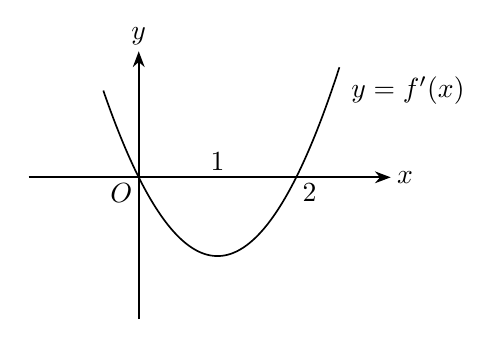
\begin{tikzpicture}[x=1cm,y=1cm,line width=0.6pt,>=Stealth,font=\normalsize]
\draw[->] (-1.4,0)--(3.2,0) node[right,inner sep=0pt,xshift=2pt] {$x$};
\draw[->] (0,-1.8)--(0,1.6) node[above,inner sep=0pt,yshift=2pt] {$y$};
\node[below left,inner sep=0pt,xshift=-2pt,yshift=-2pt] at (0,0) {$O$};
\draw[domain=-0.45:2.55,samples=100,smooth] plot (\x,{\x*(\x-2)});
\node[above,inner sep=0pt,yshift=2pt] at (1,0) {$1$};
\node[below right,inner sep=0pt,xshift=2pt,yshift=-2pt] at (2,0) {$2$};
\node[right,inner sep=0pt,xshift=4pt] at (2.55,1.1) {$y=f'(x)$};
\end{tikzpicture}
